\documentclass{beamer}
\usetheme[subsectionpage=progressbar,
	numbering=counter,
	progressbar=foot,
	]{metropolis}           % Use metropolis theme

\usepackage{hyperref}
\usepackage{graphicx}
\usepackage{url}
\usepackage{booktabs}
\usepackage[font=scriptsize,labelfont=bf]{caption}

\title{Slow rate denial of service attacks against HTTP/2 and detection}
\subtitle{Critical review}
\date{\today}
\author{Bastien Dhiver}
\institute{\href{mailto:bfrd2@kent.ac.uk}{bfrd2@kent.ac.uk}}

\begin{document}
\maketitle

\begin{frame}{Table of contents}
	\setbeamertemplate{section in toc}[sections numbered]
	\tableofcontents[hideallsubsections]
\end{frame}

\section{Authors}

\begin{frame}{Authors}

Indian Institute of Technology Indore, India

  \begin{columns}[T,onlytextwidth]
    \column{0.5\textwidth}
	\begin{figure}[t]
    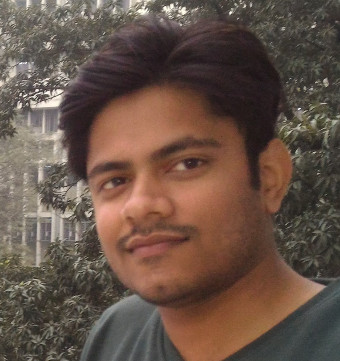
\includegraphics[width=2cm]{images/Nikhil.jpg}
    \\ Nikhil Tripathi
\centering
	\end{figure}

      \begin{itemize}
	{\small
	\item Ph.D. student
	\item Network Security, Computer Networks
	\item Slow rate DoS attacks
	}
      \end{itemize}

    \column{0.5\textwidth}

	\begin{figure}[t]
    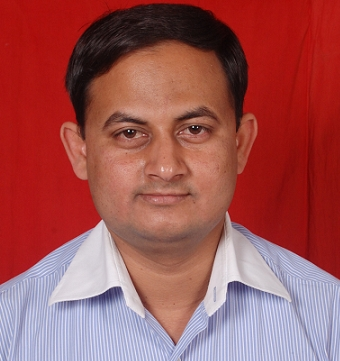
\includegraphics[width=2cm]{images/neminath.jpg}
    \\ Neminath Hubballi
\centering
	\end{figure}

      \begin{itemize}
	{\small
	\item Assistant professor
	\item Nikhil's supervisor
	\item Network Security, System Security
	\item Worked at HP, Infosys Lab, Samsung R\&D
	}
      \end{itemize}

  \end{columns}
\end{frame}

\metroset{sectionpage=none}
\section{Background}
\subsection{(Distributed) Denial-of-Service attacks}

\begin{frame}{Transport-level DDoS flooding attacks}
\begin{itemize}
	\item Exhausting network bandwidth
	\item Consumes excess amount of victim's ressources
	\item Exploiting implementation bugs of transport layer
	\item Reflection and amplification (ICMP Echo, Smurf)
	\item Require a lot of malicious client's bandwidth
	\item Can be easily detected
\end{itemize}
\end{frame}

\begin{frame}
	\begin{figure}[t]
    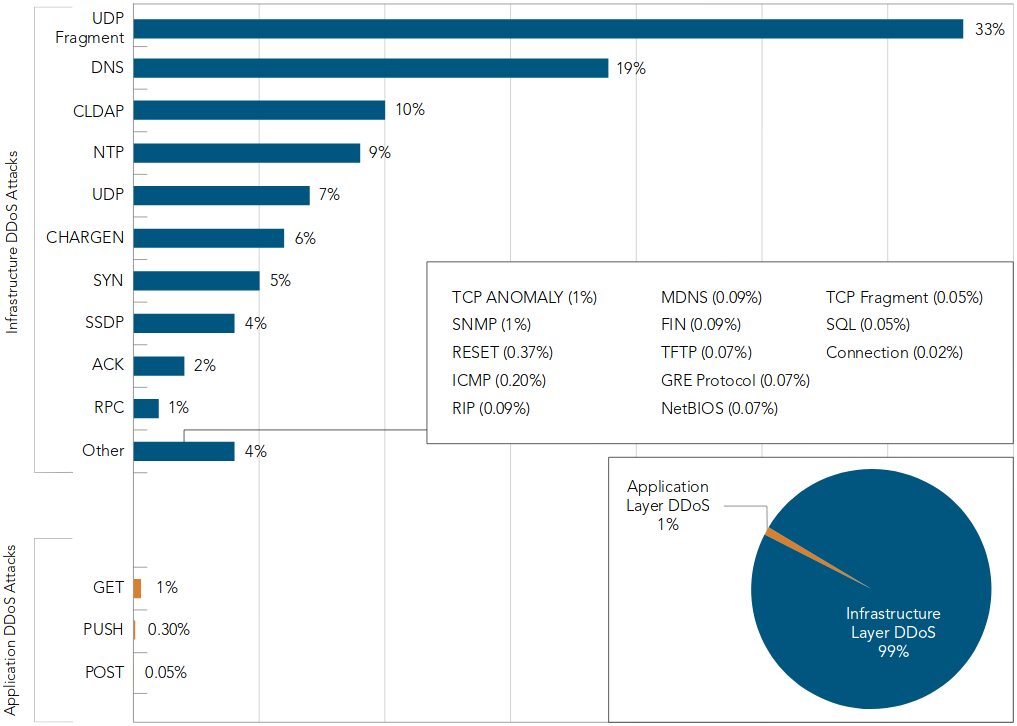
\includegraphics[scale=0.29]{images/akamai2017DDoSAttackVectorFrequency.png}
		\caption{DDoS Attack Vector Frequency, Q4 2017 from Akamai\footnote{\tiny\url{https://www.akamai.com/us/en/multimedia/documents/state-of-the-internet/q4-2017-state-of-the-internet-security-report.pdf}}}
	\end{figure}
\end{frame}

\begin{frame}{Application-level DDoS flooding attacks}
\begin{itemize}
	\item Exhausting target ressources
	\item Less bandwidth, stealthier
	\item Reflection (VoIP), Amplification (DNS), Protocol Specific (HTTP flooding)
	\item Complete requests at a very big rate
	\item Harder to distinguish from normal traffic
\end{itemize}
\end{frame}

\begin{frame}{Application-specific slow rate DoS attacks}
\begin{itemize}
	\item Very small of incomplete requests
	\item Interacts very slowly with the server
	\item Minimal bandwidth
	\item Highly stealth
	\item HTTP/1.1 Slowloris attack
	\item The proposed attacks belong to this category
\end{itemize}
\end{frame}

\begin{frame}{Application layer protocol independent slow rate DoS attacks}
  Meta attacks (FTP, SMTP, HTTP, \ldots)
  \begin{columns}[T,onlytextwidth]
    \column{0.5\textwidth}
      \begin{block}{SlowReq and SlowConn}
      \begin{itemize}
        \item Incomplete and pending requests
	\item Detect connection closes
	\item Re-establish
      \end{itemize}
	\end{block}

    \column{0.5\textwidth}
      \begin{block}{SlowNext}
      \begin{itemize}
        \item Valid and legitimate requests
	\item Maintaining established connection (keep alive)
	\item Stealth ++
      \end{itemize}
	\end{block}

  \end{columns}
\end{frame}

\subsection{HTTP/2}

\begin{frame}{{HTTP/2} in \textasciitilde one slide}
\begin{itemize}
	\item RFC 7540, May 2015
	\item Binary protocol
	\item Efficient use of TCP (one connection)
	\item Message multiplexing (frames, streams)
	\item Prediction of ressource requirement (PUSH)
	\item Header compression (HPACK)
	\item TLS as a De Facto requirement
\end{itemize}
\end{frame}

\begin{frame}{HTTP/2 frames}
\begin{columns}[T,onlytextwidth]
\column{13em}
\metroset{block=fill}

      \begin{block}{Connection Preface}
        Initial settings for a HTTP/2 connection
      \end{block}

      \begin{block}{WINDOW\_UPDATE}
        Number of bytes that the sender is willing to accept
      \end{block}

      \begin{block}{GOAWAY}
	\begin{itemize}
        	\item Indicate to tear off an established connection
		\item Carry an error code
	\end{itemize}
      \end{block}

\column{13em}
\metroset{block=fill}
      \begin{block}{HEADERS and CONTINUATION}
        Transmit the headers
      \end{block}

      \begin{block}{DATA}
        Carry message body
	\end{block}

      \begin{block}{SETTINGS}
        Negotiate connection parameters
	\begin{itemize}
		\item Initial window size
		\item Max concurent streams
	\end{itemize}
      \end{block}

\end{columns}
\end{frame}

\begin{frame}{Multiplexing}
  \begin{figure}[t]
    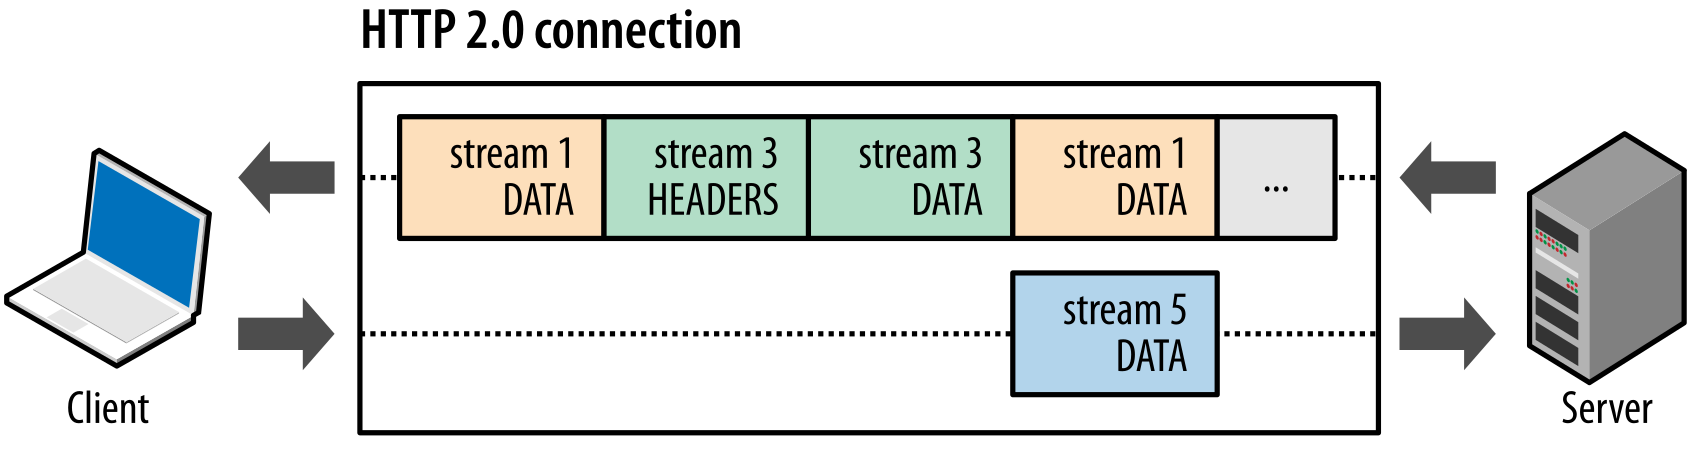
\includegraphics[scale=0.22]{images/http2Conn.png}
	  \caption{HTTP/2 request and response multiplexing within a shared connection~\cite{Grigorik:2013}}
  \end{figure}
	HTTP/1.1 HoL (Head-of-line) blocking solved
\end{frame}

\begin{frame}{In real life?}
  \begin{figure}[t]
    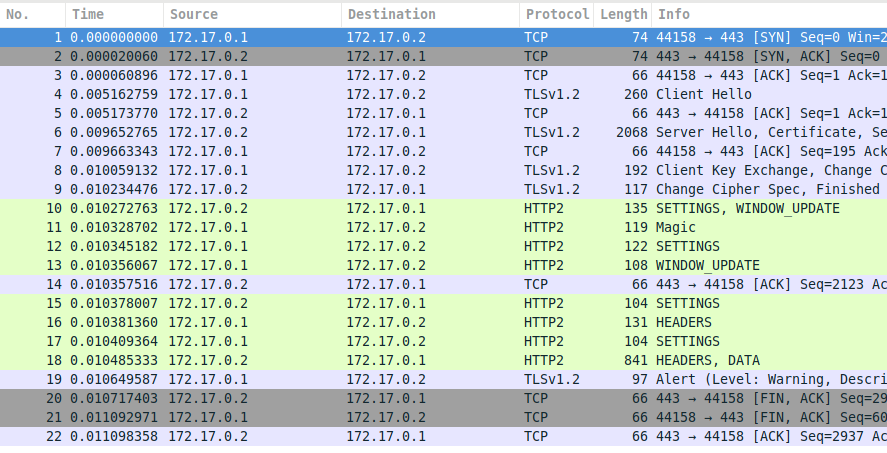
\includegraphics[scale=0.35]{images/HTTP2BasicExchangeNginxCurl.png}
	  \caption{Decrypted HTTP/2 exchange between Nginx and curl displayed in Wireshark}
  \end{figure}
	The client IP address is 172.17.0.\textbf{1}\hspace{10em}\tiny EZPZ
\end{frame}

\section{The paper \cite{Tripathi:2018}}

\subsection{Proposed attacks}

\begin{frame}{Proposed attacks}
\begin{itemize}
	\item Five novel Slow Rate HTTP/2 DoS attacks
	\item Number of \textbf{free connections slots} available is targeted
	\item \textbf{Hold back} established connections for a long duration
	\item Tested on four popular web servers
\end{itemize}
	\begin{center}Apache, Nginx, H2O and Nghttp2\end{center}
\end{frame}

\begin{frame}{Attack \textnumero 1}
  \begin{figure}[t]
    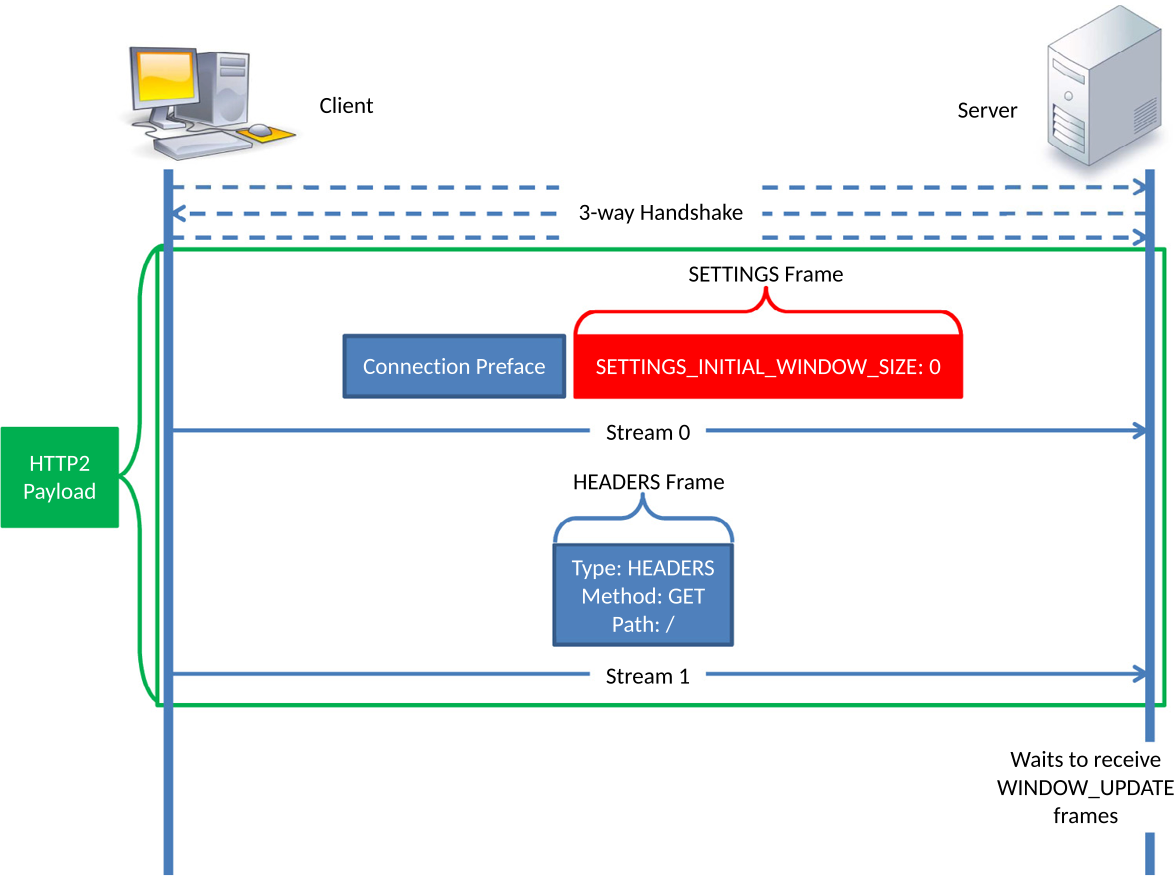
\includegraphics[scale=0.22]{images/attack1.png}
    \caption{Attack-1. SETTINGS frame with INITIAL\_WINDOW\_SIZE set to 0}
  \end{figure}
\end{frame}

\begin{frame}{Attack \textnumero 2}
  \begin{figure}[t]
    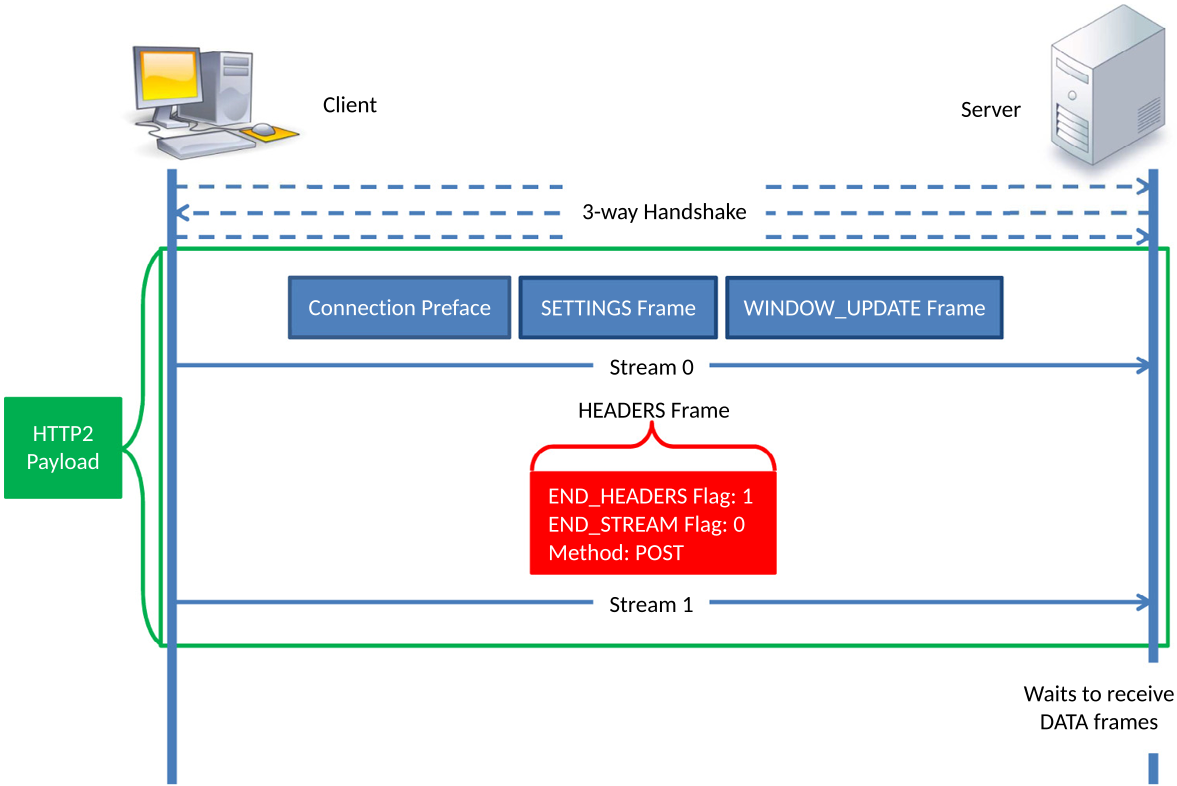
\includegraphics[scale=0.24]{images/attack2.png}
    \caption{Attack-2. HEADERS frame with END\_HEADERS set and END\_STREAM reset}
  \end{figure}
\end{frame}

\begin{frame}{Attack \textnumero 3}
  \begin{figure}[t]
    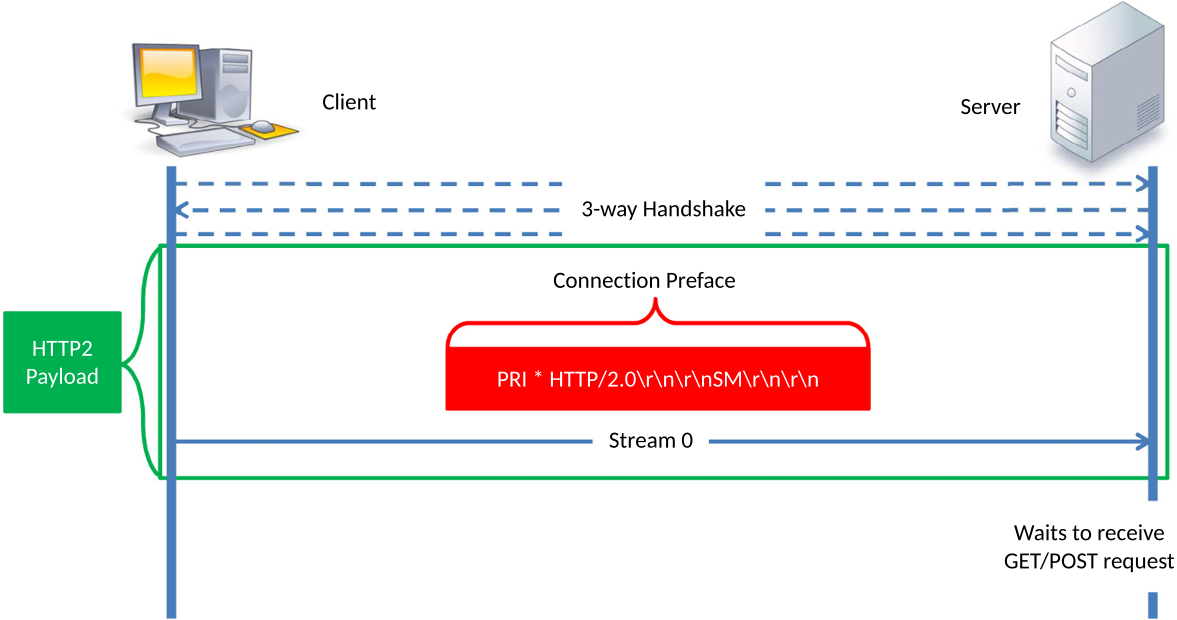
\includegraphics[scale=0.26]{images/attack3.png}
    \caption{Attack-3. First HTTP/2 payload with only Connection Preface}
  \end{figure}
\end{frame}

\begin{frame}{Effects}
\begin{table}
    \caption{Connection waiting time in seconds and \textnumero~at servers for the five attacks}
    \begin{tabular}{@{} lr c c c c c c @{}}
      \toprule
	    Server & A1 & A2 & A3 & A4 & A5 & \textnumero~conn\\
      \midrule
	    Apache & 300 & 600-$\infty$ & 300-300 & 300-$\infty$ & 5-5 & 150\\
	    Nginx & 60 & 30-$\infty$ & 30-$\infty$ & 90-90 & 180-180 & 2060\\
	    H2O & $\infty$ & 10-$\infty$ & 10-10 & 10-$\infty$ & 10-10 & 1024\\
	    Nghttp2 & 60 & 10-975 & 10-975 & 10-60 & 10-975 & 1142\\
      \bottomrule
    \end{tabular}
\end{table}
	\begin{alertblock}{Same effects over TLS}\end{alertblock}
\end{frame}

\subsection{Proposed detection mechanism}

\begin{frame}{Chi-square test}
	Distance measurement technique
  \begin{columns}[T,onlytextwidth]
    \column{0.5\textwidth}
\begin{figure}
	\[{\chi}^2 = \sum_{i=1}^{n} \frac{(O_i - E_i)^2}{E_i}\]
		\caption{Chi-square equation}
\end{figure}
\begin{alertblock}{To be set}
	\begin{itemize}
		\item Feature selection
		\item Significance level $\alpha$
	\end{itemize}
\end{alertblock}
    \column{0.6\textwidth}
	  \vspace{2.3em}
	  $n$: Number of categories\\
	  $O_i$: Observed cases in $i_\text{th}$ category\\
	  $E_i$: Expected cases in $i_\text{th}$ category\\
	  $i$: number of the category\\
  \end{columns}
\end{frame}

\begin{frame}{How does it work?}
  \begin{figure}[t]
    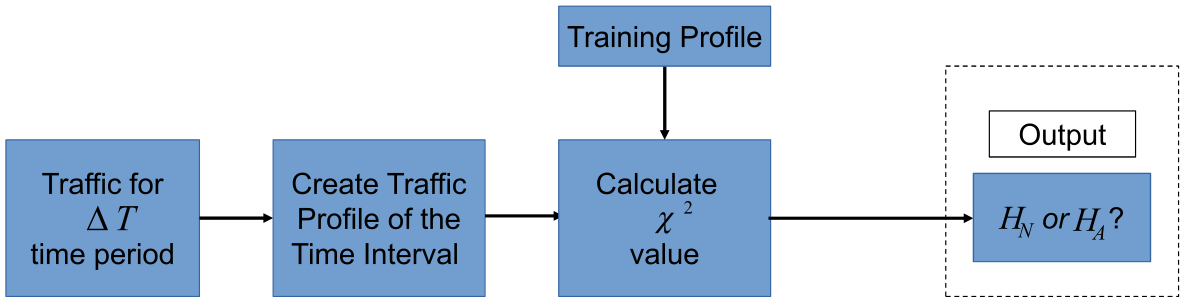
\includegraphics[scale=0.26]{images/detector.png}
    \caption{Detector working}
  \end{figure}
	Training and testing phases
\end{frame}

\begin{frame}{Detection performance}
  \begin{figure}[t]
    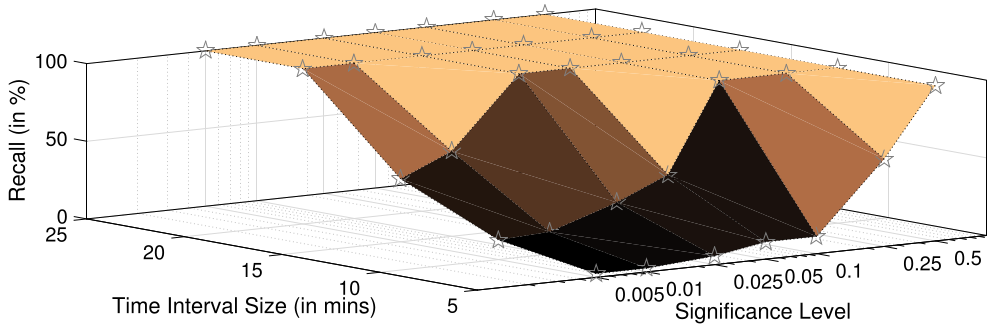
\includegraphics[scale=0.27]{images/recallRate.png}
    \caption{Recall rate}
  \end{figure}
	\vspace{-1.5em}
  \begin{figure}[t]
    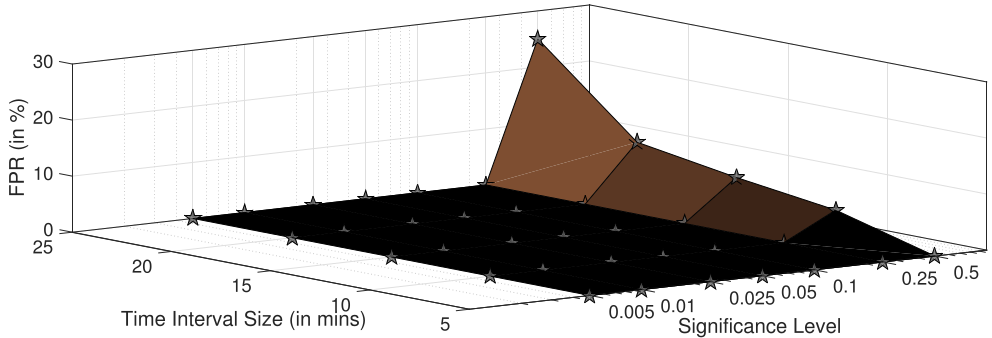
\includegraphics[scale=0.27]{images/falsePositiveRate.png}
    \caption{False positive rate}
  \end{figure}
\end{frame}

\metroset{sectionpage=progressbar}
\section{Prior work}
\begin{frame}{Prior work}
	\begin{alertblock}{Vulnerabilities in HTTP/2 protocol}
	\begin{itemize}
		\item Two papers by Adi and al~\cite{Adi:2015} \cite{Adi:2016}
		\item Flood attack, reduction of Quality (RoQ) only
		\item Impreva report
		\item Slow Read, HPACK, Dependency DoS, Stream abuse \Rightarrow patched
	\end{itemize}
	\end{alertblock}
	\begin{alertblock}{Anomalies in encrypted network traffic}
	\begin{itemize}
		\item Observing inter-packet arrival time, time gaps, \ldots
	\end{itemize}
	\end{alertblock}
	\begin{alertblock}{Chi-square test}
	\begin{itemize}
		\item Used to detect intrusion, port scan, bot servers (C2)
	\end{itemize}
	\end{alertblock}
\end{frame}

\section{Applicability of research}
\begin{frame}{Applicability of research}
\begin{itemize}
	\item Submitted in 2017, published in 2018 (ACM)
	\item HTTP/2 deployement $\nearrow$
	\item Real web servers used
	\item Real effects shown
	\item Credible testbed
\end{itemize}
\end{frame}

\section{Criticisms}

\begin{frame}{Proof-of-Concept}
	\begin{itemize}
		\item "we implemented these attacks in python"\ldots
		\item I implemented them
		\item Published soon
		\item Serveral differences with the authors' results
	\end{itemize}
  \begin{figure}[t]
    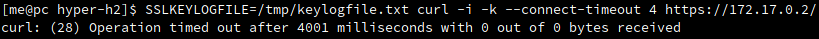
\includegraphics[scale=0.38]{images/curlTimout.png}
    \caption{An effective attack caused curl connection timeout}
  \end{figure}
\end{frame}

\begin{frame}{Erwin Adi Ph.D. Thesis}
	\begin{quote}
"Denial-of-service attack modelling and detection for HTTP/2 services" ~\cite{Adi:2017}
	\end{quote}
\begin{itemize}
	\item Four novel attacks
	\item Flood attacks
	\item Four machine learning techniques used (suitable for detection)
	\item Features used: number of connections, flow information, \ldots
\end{itemize}
\end{frame}

\begin{frame}{Personnal opinion}
\begin{itemize}
	\item Where are the Proofs-of-Concept??
	\item Examples shown with HTTP/2 plaintext protocol $\ne$ real life
	\item Only chi-square statistical test is mentionned
	\item Very specific to HTTP/2
	\item Good idea to focus on the number of available slot connection
\end{itemize}
\end{frame}

\begin{frame}[standout]
	Thank you! 
\end{frame}
\begin{frame}[standout]
	Thank you! 
	
\includegraphics[scale=0.3]{images/ok-hand.png}
\end{frame}

\appendix

\begin{frame}{Attack \textnumero 4}
  \begin{figure}[t]
    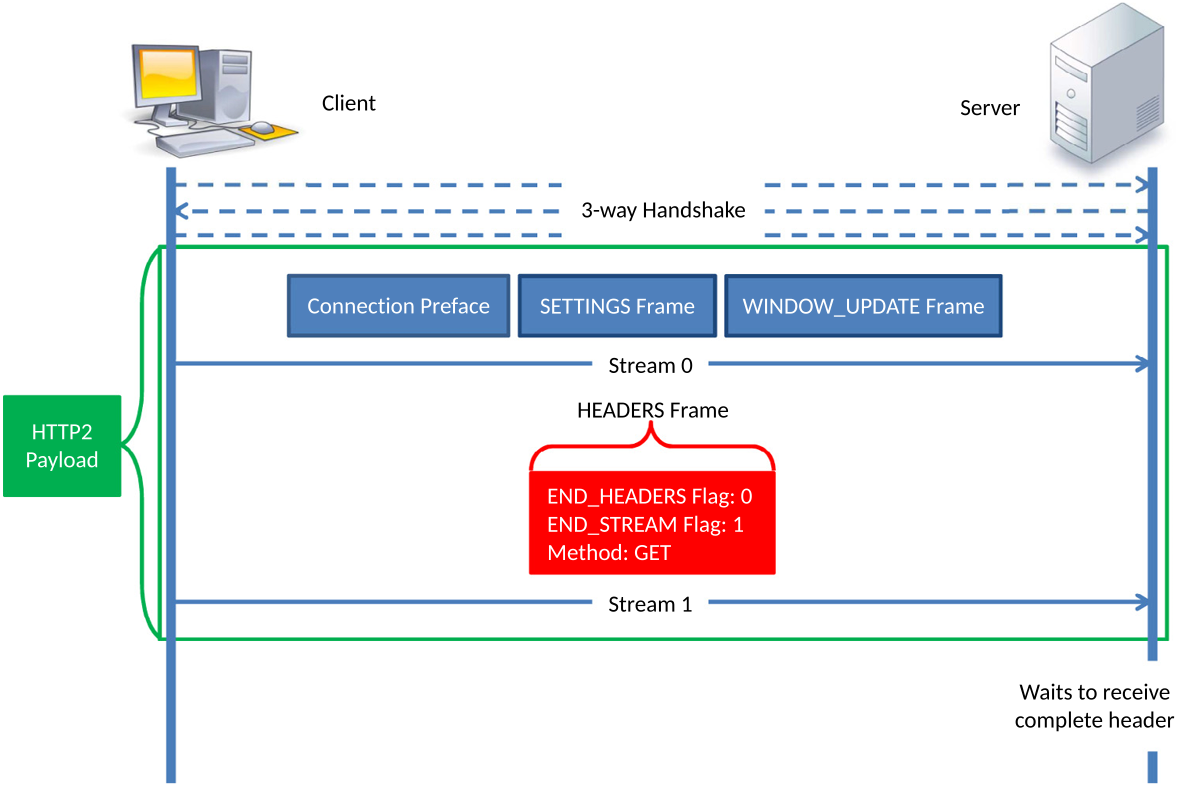
\includegraphics[scale=0.22]{images/attack4.png}
    \caption{Attack-4. HEADERS frame with END\_HEADERS reset and END\_STREAM set}
  \end{figure}
\end{frame}

\begin{frame}{Attack \textnumero 5}
  \begin{figure}[t]
    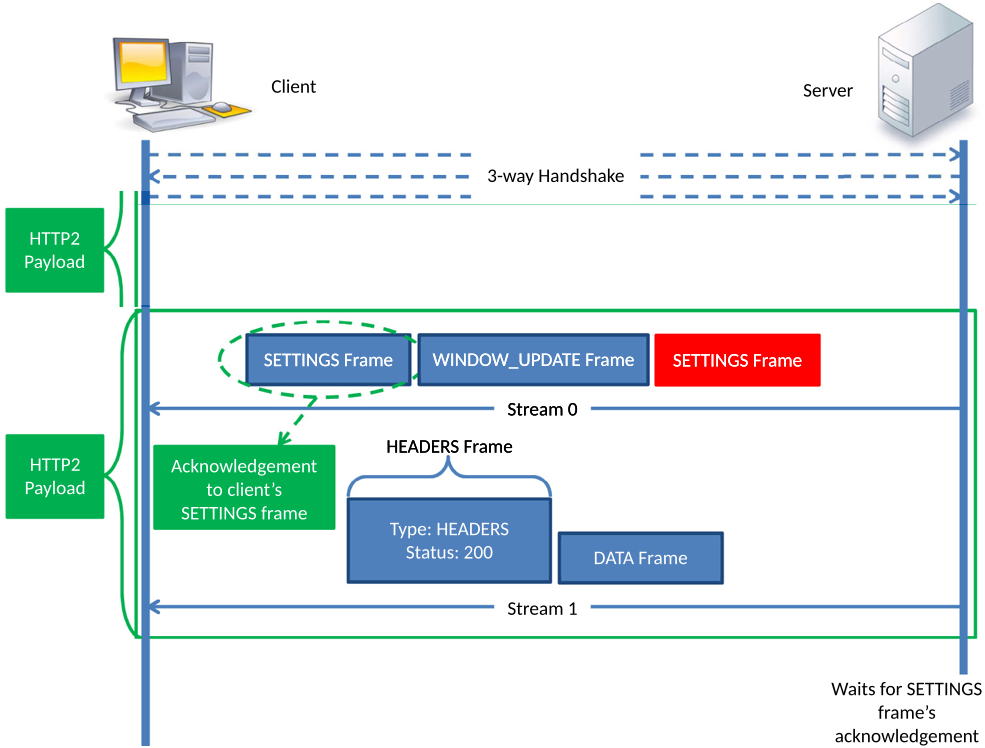
\includegraphics[scale=0.27]{images/attack5_short.png}
    \caption{Attack-5. Client never acknowledges SETTINGS frame sent by server}
  \end{figure}
\end{frame}

\begin{frame}{Web servers usage}
	Accessed: 21 Febuary 2018
  \begin{columns}[T,onlytextwidth]
    \column{0.5\textwidth}
	  \vspace{2em}
	  \begin{figure}[t]
	    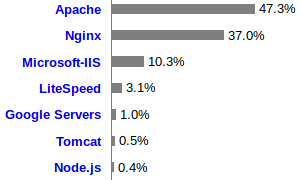
\includegraphics[scale=0.45]{images/w3techsWebServersUsage.png}
		  \caption{\href{https://w3techs.com/technologies/overview/web\_server/all}{Market share of active sites by W3Techs.com}}
	  \end{figure}
    \column{0.5\textwidth}
	  \begin{figure}[t]
	    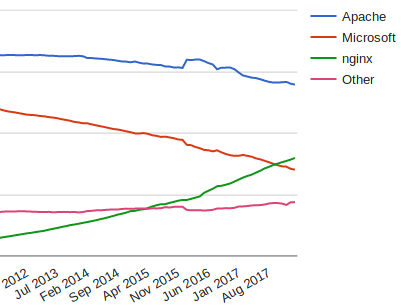
\includegraphics[scale=0.4]{images/netcraftWebServersUsage.png}
		  \caption{\href{https://news.netcraft.com/archives/2018/02/13/february-2018-web-server-survey.html}{Percentages of websites using various web servers by Netcraft}}
	  \end{figure}
  \end{columns}
\end{frame}

\begin{frame}{HTTP/2 websites adoption}
	Accessed: 21 Febuary 2018
	  \begin{figure}[t]
		  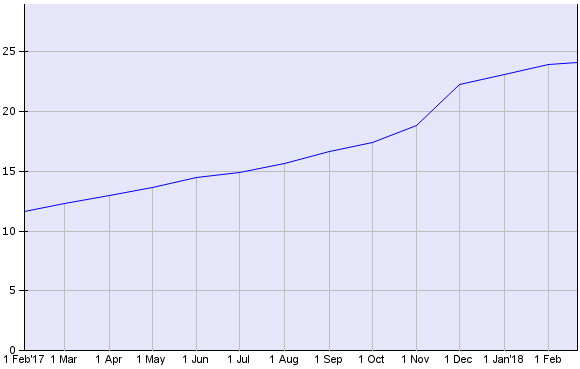
\includegraphics[scale=0.4]{images/http2WebsitesUsage.png}
		  \caption{\href{https://w3techs.com/technologies/details/ce-http2/all/all}{Usage of HTTP/2 for websites by W3Techs.com}}
	  \end{figure}
\end{frame}

\begin{frame}{Can I use HTTP/2?}
	Accessed: 21 Febuary 2018
	  \begin{figure}[t]
	          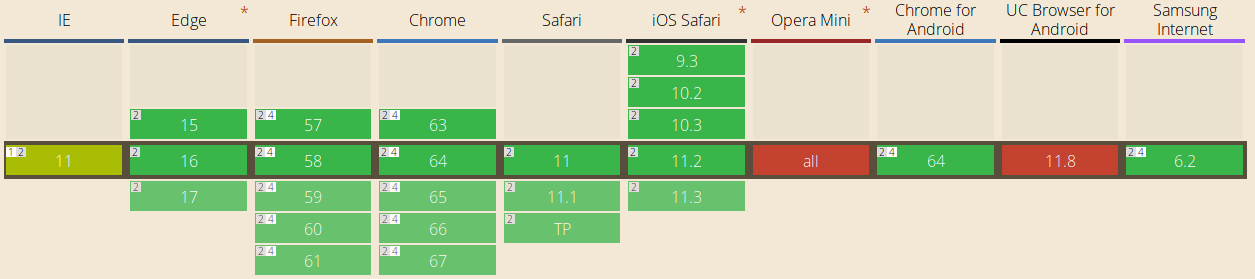
\includegraphics[scale=0.25]{images/canIUseHTTP2.png}
	          \caption{\href{https://caniuse.com/\#feat=http2}{HTTP/2 capable clients by caniuse.com}}
	  \end{figure}
\end{frame}

\begin{frame}[allowframebreaks]{References}

  \bibliography{refs}
  \bibliographystyle{unsrt}

\end{frame}

\end{document}
